\documentclass[11pt]{article}

%% Page Margins %%
\usepackage{geometry}
\geometry{
    top = 0.9in,
    bottom = 0.9in,
    right = 0.9in,
    left = 0.9in,
}

\usepackage[utf8]{inputenc}
\usepackage[T1]{fontenc}
\usepackage{amsmath}
\usepackage{graphicx}
\usepackage{booktabs}
\usepackage{parskip}
\usepackage{xcolor}
\usepackage{enumitem}
\usepackage[numbers,sort&compress]{natbib}
\usepackage[hidelinks]{hyperref}
\usepackage{caption}
\captionsetup{font=small,labelfont=bf}

\definecolor{helps}{HTML}{2A78D6}
\definecolor{hurts}{HTML}{E34948}
\definecolor{muted}{HTML}{7C838B}
\definecolor{boxbg}{HTML}{F4F6F8}

\newcommand{\cond}[1]{\texttt{#1}}
\newcommand{\yes}[1]{\textcolor{helps}{#1}}
\newcommand{\no}[1]{\textcolor{hurts}{#1}}

% simple grey box for the reading guide
\newcommand{\guidebox}[1]{%
  \noindent\colorbox{boxbg}{\parbox{\dimexpr\linewidth-2\fboxsep}{\small #1}}\par\medskip}

\title{Can a Transformer Learn a Teacher's Board and Voice Together?\\[6pt]
\large Building a stroke+speech dataset from 1,191 lecture videos, and measuring whether the two modalities help each other}
\author{Taehyeon Kim}
\date{September 2026}

\begin{document}
\maketitle

\begin{abstract}
A math teacher on YouTube writes on the board and talks at the same time. I wanted to know whether a model can learn both from video --- and, more specifically, whether the writing helps predict the speech and the speech helps predict the writing. To find out, I built a pipeline that turns 1,191 lecture videos into an aligned sequence of spoken words and pen movements (12.5M tokens), trained one small transformer on that sequence, and ran a controlled experiment that removes one kind of context at a time. The result: the board \emph{does} help predict the next word (a robust $+0.125$ nats), but putting pen movements into the same sequence as the words costs more than that help is worth ($-0.42$ nats), and the speech does not help predict the pen at all. In plain terms: the two signals are related, but mixing them into one stream is the wrong way to use that relationship at this scale. That finding points to the next design, where a language agent plans what to say and what to draw, and a separate renderer puts it on the board.
\end{abstract}

\section{The question}

Watch The Organic Chemistry Tutor explain fractions. He says ``two fifths plus one fourth'' while writing $\tfrac{2}{5} + \tfrac{1}{4}$. The words and the pen are clearly related. My question was whether that relationship is something a model can \emph{use}:

\begin{quote}
Does what is already on the board tell you the next word he will say? Does what he has said tell you the next pen movement?
\end{quote}

If both are yes, one model can take the board and the speech as shared context and produce both. If not, the two should be handled separately. This report is the experiment that decides.

Nobody had tested this on real teaching video. The closest existing system plans whiteboard content with a vision-language model from 24 hand-made demonstrations and renders it in sync with narration~\citep{prasad2026whiteboard}; it does not learn from a real teacher. So the first job was to build the data.

\section{What others have done}

\textbf{Making a machine write by hand.} The standard recipe is a sequence model that emits pen movements one point at a time, where each output is not a single point but a \emph{mixture of Gaussians} over where the pen might go next~\citep{bishop1994mdn}. Graves showed this produces convincing cursive when the model is also told which characters to write~\citep{graves2013generating}; that work trained on IAM-OnDB, about 86k words from 200+ writers captured on a whiteboard~\citep{liwicki2005iamondb}. Sketch-RNN applied the same output head to drawings, with the pen encoded as $(\Delta x, \Delta y, \text{pen state})$~\citep{ha2018sketchrnn} --- the format this report uses. Later work separates \emph{what} is written from \emph{how} it is written~\citep{aksan2018deepwriting}, or replaces the point-by-point model with diffusion over whole strokes~\citep{pan2026diffink,zhou2025strokefusion}, or tokenizes ink so an ordinary language model can consume it~\citep{wang2026scribetokens}, or skips the pen entirely and generates the act of sketching as video~\citep{ren2026videosketcher}. A dataset of 230k handwritten math expressions exists for recognition~\citep{gervais2024mathwriting}, but it has no speech and no timing.

\textbf{Getting handwriting out of lecture video.} Detecting and binarizing what a teacher wrote on a whiteboard in a fixed-camera lecture video is a studied problem~\citep{davila2017whiteboard,kota2019lecture}. Those systems produce the final image on the board; this project additionally needs the \emph{order and timing} of every stroke, so it can be lined up with the speech.

\textbf{Putting two kinds of tokens in one transformer.} Large multimodal models have gone both ways. Chameleon puts images and text into a single token sequence and trains on it from scratch at 7--34B parameters~\citep{chameleon2024}. Flamingo keeps the language model's sequence pure and lets it look at visual features through separate cross-attention layers~\citep{alayrac2022flamingo}. The experiment in this report is, in miniature, a comparison of those two philosophies for speech and pen.

\textbf{Language models that draw.} A recent line of work has a language model output a \emph{plan} for a picture --- element types and coordinates --- and renders it: diagrams~\citep{zala2024diagrammergpt}, scene layouts~\citep{feng2023layoutgpt}, scientific figures as TikZ code~\citep{belouadi2024automatikz}, and sketches drawn stroke by stroke on a numbered grid with no training at all~\citep{vinker2024sketchagent}. The next step proposed at the end of this report belongs to this family.

\section{Data: turning videos into a training sequence}
\label{sec:data}

This was most of the work. No dataset of ``what a teacher says and draws, aligned in time'' exists, so I built one.

\subsection{Pipeline}

Each video goes through six stages (Figure~\ref{fig:pipeline}):

\begin{enumerate}[leftmargin=*,itemsep=2pt]
\item \textbf{Download} the video and audio.
\item \textbf{Frames.} Extract frames at 30\,fps.
\item \textbf{Stroke extraction.} Detect newly deposited ink between frames, thin it to a skeleton, and track the pen tip. Output: strokes as lists of $(x, y, t)$ points, subsampled to 10\,fps. Coordinates are normalized to $[0,1]$ over the $1280 \times 720$ canvas. This is the same detection problem as in lecture-video summarization~\citep{davila2017whiteboard,kota2019lecture}, but keeping the temporal order of the ink rather than only the final image.
\item \textbf{Speech to text.} Whisper~\citep{radford2023whisper} on the audio track gives every word with a start and end time.
\item \textbf{Merge.} Words and strokes are interleaved into one time-ordered event stream.
\item \textbf{Align.} Each stroke is attached to the word being spoken while it was drawn (maximum time overlap). Strokes drawn while nobody is speaking are attached to a \cond{<silent>} token.
\end{enumerate}

\begin{figure}[ht!]
\centering
\small
\begin{tabular}{c}
\texttt{video} $\;\rightarrow\;$ \texttt{frames (30 fps)} $\;\rightarrow\;$ \texttt{stroke extraction} $\;\rightarrow\;$ \texttt{strokes.jsonl} \\[4pt]
\texttt{audio} $\;\rightarrow\;$ \texttt{Whisper} $\;\rightarrow\;$ \texttt{words.jsonl} \\[4pt]
\texttt{strokes + words} $\;\rightarrow\;$ \texttt{merge} $\;\rightarrow\;$ \texttt{align} $\;\rightarrow\;$ \texttt{training.jsonl}
\end{tabular}
\caption{The data pipeline. One command runs it end to end for a YouTube URL.}
\label{fig:pipeline}
\end{figure}

The pipeline ran across 8--12 lab machines in parallel. (Scaling to 30 machines triggered YouTube rate limiting, so 8--12 is the practical ceiling.) The manifest had 1,372 videos; 1,191 completed cleanly.

\subsection{Why this teacher}

The Organic Chemistry Tutor writes slowly and deliberately, one symbol at a time, with clear gaps between strokes. That makes extraction reliable. Cursive-style teachers (Khan Academy) were tried and deferred: the cursor and freshly deposited ink overlap at the pen tip, and the reconstructions were unreadable.

\subsection{What the data looks like}

Before training anything I measured the corpus, and several numbers changed the design (Table~\ref{tab:data}). For scale: the 9.7M pen points here are more than the whole of IAM-OnDB, the dataset the classic handwriting-synthesis results were trained on~\citep{liwicki2005iamondb,graves2013generating}, and they all come from one writer.

\begin{table}[ht!]
\centering
\small
\begin{tabular}{@{}l r l@{}}
\toprule
& value & why it matters \\
\midrule
videos / pages & 1,191 / 1,191 & every video is one board; no board-clear events survived \\
total tokens & 12.5M & \\
\quad pen points & 9.7M (78\%) & the sequence is mostly pen \\
\quad words & 2.77M (22\%) & \\
vocabulary & 5,525 & after lower-casing and stripping Whisper's punctuation (was 11k) \\
median page & 8,860 tokens & 95\% of pages are longer than a 1,024-token window \\
points per stroke & median 6 & 10\,fps sampling; a letter is a handful of points \\
drawing that starts from \cond{<silent>} & 49\% & half of all writing happens with nobody talking \\
within-stroke step & median 0.006 & tiny \\
between-stroke jump & median 0.04, 90th pct 0.30 & large; pen motion is two very different distributions \\
\bottomrule
\end{tabular}
\caption{The corpus after the pipeline. Distances are in normalized canvas units.}
\label{tab:data}
\end{table}

Two of these directly shaped the model. The bimodal pen motion (tiny steps within a stroke, big jumps between strokes) is why the output head is a mixture of Gaussians rather than a single predicted point. The 49\% of drawing that starts from \cond{<silent>} is why that token must be allowed at generation time --- an earlier version banned it and could barely draw.

\section{The model, in plain terms}

One transformer~\citep{vaswani2017attention} reads the lecture as a single sequence of tokens in the order they happened:
\begin{center}
\texttt{[today] [we] [have] [pen] [pen] [pen] [a] [squared] [pen] [<silent>] [pen] \ldots}
\end{center}
A word token carries a word. A pen token carries where the pen moved ($dx$, $dy$) and whether it lifted, following the Sketch-RNN encoding~\citep{ha2018sketchrnn}. At every position the model predicts what comes next. Since the next thing can be a word or a pen move, it has three small output heads: one that decides \emph{which kind} comes next, one that picks the word, and one that says where the pen goes.

The pen head predicts a \emph{distribution} of possible next moves (20 overlapping Gaussian blobs), not a single point --- a mixture density network~\citep{bishop1994mdn,graves2013generating}. If you only predict one point, you get the average of ``curve left'' and ``curve right'', which is ``stay still'', and the strokes collapse into dots. That is exactly what the earlier attempts on this project produced.

The model is small on purpose: 4.6M parameters, 20 epochs, about six minutes per training run on a free Colab GPU. The goal was a clean comparison between conditions, not a strong model.

\guidebox{%
\textbf{Details for reproduction.} 4 layers, model width 256, 8 attention heads, pre-norm layout~\citep{xiong2020prenorm}, GELU activations~\citep{hendrycks2016gelu}, sinusoidal position encoding~\citep{vaswani2017attention}, context window 1,024 tokens. Trained with AdamW~\citep{loshchilov2019adamw} at learning rate $3\times10^{-4}$ with a 200-step warm-up and cosine decay, batch size 8, mixed precision~\citep{micikevicius2018mixed}, label smoothing 0.1 on the word head~\citep{szegedy2016inception}. Pen coordinates are deltas scaled by 20 so their standard deviation ($\approx 1.25$) matches the mixture's initial width.}

\guidebox{%
\textbf{How to read the numbers.} Every result below is a \emph{loss}: how surprised the model was by what actually came next, averaged over the held-out lectures. Lower is better. Word loss is in \emph{nats}; $e^{\text{loss}}$ is the \emph{perplexity}, roughly ``how many words the model was choosing between'' --- perplexity 47 means it had narrowed the next word down to about 47 candidates. Pen loss is also in nats but can be negative, because it is the log of a probability density rather than a probability. A difference of 0.1 nats between two conditions is large: it is the difference between perplexity 47 and 52. Every number is the mean over three separately trained models (three random seeds), and a result is only called \emph{robust} when all three seeds agree.}

\section{How I measured it}
\label{sec:measure}

The idea is simple: keep everything the same and take away one kind of context at a time, then see how much worse the prediction gets. To test ``does the board help the next word'', the conditions are:

\begin{center}
\small
\begin{tabular}{@{}l l@{}}
\toprule
\cond{full}            & the model sees the words and the real pen movements \\
\cond{mask\_strokes}   & the pen tokens are there, but their coordinates are zeroed out \\
\cond{nostroke\_hidden}& the pen tokens are there but hidden from attention entirely \\
\cond{drop\_strokes}   & the pen tokens are removed; the model sees only words \\
\bottomrule
\end{tabular}
\end{center}

Each step down removes one thing: first the pen \emph{content}, then the fact that a pen event \emph{happened}, then the empty \emph{space} the pen tokens took up. Reading the word loss at each step tells you what each of those was worth. The same ladder in the other direction (\cond{mask\_words}, \cond{noword\_hidden}, \cond{drop\_words}) tells you what the speech is worth for predicting the pen.

All conditions are evaluated on exactly the same 363 held-out windows, so the comparison is fair.

\subsection{Two things I had to fix along the way}

\textbf{The first version compared the wrong things.} It only had \cond{mask} and \cond{drop}. But removing the pen tokens also shrinks the window to a quarter of its length and pushes the words right next to each other, so ``drop minus mask'' mixed two effects: losing the pen information, and changing the spacing. The \cond{hidden} condition was added to separate them --- same length, same spacing, pen slots simply invisible.

\textbf{One training run is not enough.} Training the same condition twice with the same seed gave losses of 4.22 and 4.36. GPU arithmetic in half precision is not deterministic, and a small model amplifies the difference. That the random seed alone can move results by more than the effect being studied is well documented~\citep{picard2021seed,bouthillier2021variance}, and the 0.14-nat gap here is bigger than most of the effects I was measuring. So every condition was trained three times and I only trust a result all three agree on. Within each run, the uncertainty is a bootstrap~\citep{efron1979bootstrap} over held-out \emph{windows} rather than tokens, because tokens from the same lecture are not independent.

\section{Results}

Figure~\ref{fig:ladder} and Table~\ref{tab:ladder} show the loss at every step of both ladders.

\begin{figure}[ht!]
    \centering
    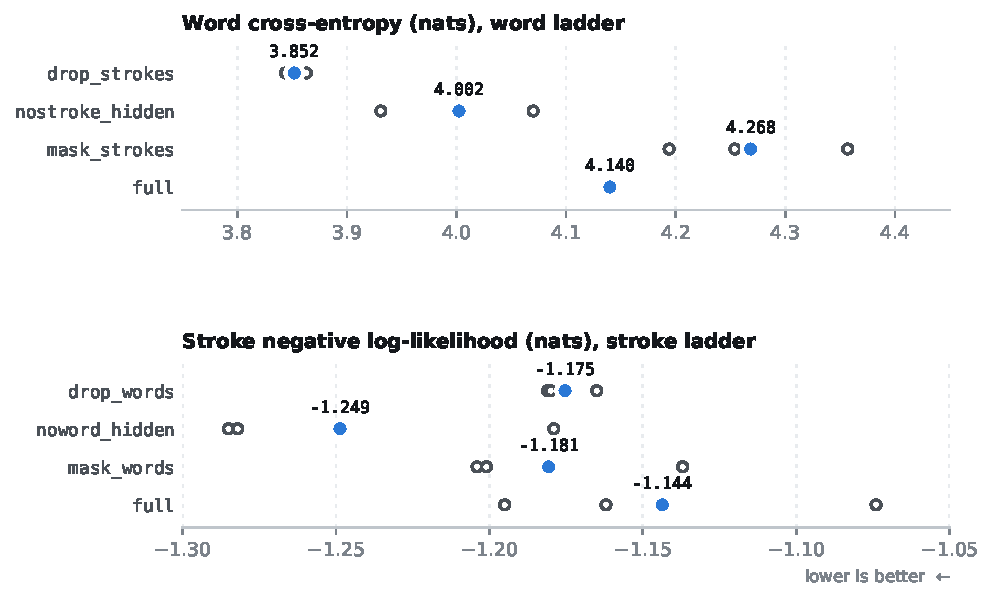
\includegraphics[width=0.92\textwidth]{fig/ladder.pdf}
    \caption{Loss at each condition. Filled marks are the mean of three seeds; hollow dots are the individual seeds. \textbf{Top:} the word ladder runs backwards --- the less pen information the model sees, the better it predicts words. \textbf{Bottom:} the stroke ladder is nearly flat; the four conditions sit within 0.1 nats and the seeds overlap.}
    \label{fig:ladder}
\end{figure}

\begin{table}[ht!]
    \centering
    \small
    \begin{tabular}{@{}l r r r@{}}
    \toprule
    condition & word loss & perplexity & pen loss \\
    \midrule
    \cond{full}             & $4.140 \pm 0.003$ & 62.8 & $-1.144 \pm 0.063$ \\
    \cond{mask\_strokes}    & $4.268 \pm 0.082$ & 71.4 & $-0.741 \pm 0.023$ \\
    \cond{nostroke\_hidden} & $4.002 \pm 0.070$ & 54.7 & --- \\
    \cond{drop\_strokes}    & $3.852 \pm 0.010$ & 47.1 & --- \\
    \cond{mask\_words}      & $4.384 \pm 0.002$ & 80.2 & $-1.181 \pm 0.038$ \\
    \cond{noword\_hidden}   & --- & --- & $-1.249 \pm 0.061$ \\
    \cond{drop\_words}      & --- & --- & $-1.175 \pm 0.009$ \\
    \bottomrule
    \end{tabular}
    \caption{Held-out loss, mean $\pm$ std over three seeds. The word-only model (\cond{drop\_strokes}) predicts words best.}
    \label{tab:ladder}
\end{table}

The numbers that answer the question are the \emph{differences between neighbouring steps}, because each one isolates a single effect. Figure~\ref{fig:deltas} and Table~\ref{tab:deltas} show them as ``how much the loss went down when this information was added'', so a positive number means it helped.

\begin{figure}[ht!]
    \centering
    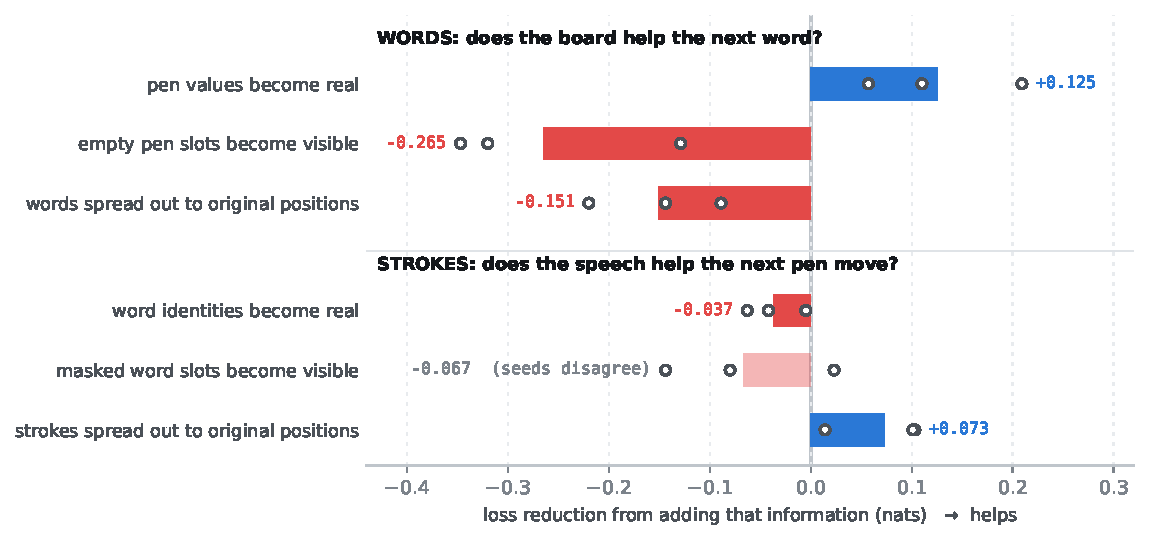
\includegraphics[width=0.92\textwidth]{fig/deltas.pdf}
    \caption{What each kind of context is worth. Blue bars helped, red bars hurt. Hollow dots are the three seeds. Every bar except one has all three seeds on the same side of zero.}
    \label{fig:deltas}
\end{figure}

\begin{table}[ht!]
    \centering
    \small
    \begin{tabular}{@{}l r r l@{}}
    \toprule
    what was added & $\Delta$ (nats) & per seed & verdict \\
    \midrule
    \multicolumn{4}{@{}l}{\textit{Words: does the board help the next word?}} \\
    real pen coordinates            & $\mathbf{+0.125 \pm 0.077}$ & $+0.21 / +0.06 / +0.11$ & \yes{robust, helps} \\
    empty pen slots become visible  & $-0.266 \pm 0.119$ & $-0.35 / -0.13 / -0.32$ & \no{robust, hurts} \\
    words spread to original spacing& $-0.151 \pm 0.066$ & $-0.14 / -0.22 / -0.09$ & \no{robust, hurts} \\
    \addlinespace
    \multicolumn{4}{@{}l}{\textit{Strokes: does the speech help the next pen move?}} \\
    real word identities             & $-0.037 \pm 0.029$ & $-0.04 / -0.01 / -0.06$ & \no{robust, hurts a little} \\
    masked word slots become visible & $-0.067 \pm 0.084$ & $-0.08 / +0.02 / -0.14$ & \textcolor{muted}{seeds disagree} \\
    strokes spread to original spacing & $+0.073 \pm 0.051$ & $+0.10 / +0.01 / +0.10$ & \textcolor{muted}{robust, but see \S\ref{sec:limits}} \\
    \bottomrule
    \end{tabular}
    \caption{Each step of the ladder as a loss reduction. \emph{Robust} means all three seeds agree in sign and each seed's confidence interval (bootstrapped over held-out windows) excludes zero.}
    \label{tab:deltas}
\end{table}

\section{What it means}

\textbf{1. Yes --- the board tells you the next word.} Giving the model the real pen coordinates instead of zeros makes its word predictions better by $0.125$ nats, in every seed. This is the cleanest comparison in the whole design: the two sequences are identical token for token, only the pen numbers differ. When the pen is drawing a fraction bar, ``over'' becomes more likely, and the model learned that.

\textbf{2. But putting the pen in the same sequence costs more than that.} Two separate costs showed up. Simply having the pen slots \emph{visible} --- even with no information in them --- costs $0.266$ nats. Attention spreads across everything it can see, and when 78\% of the sequence is pen tokens, most of it is spent on tokens that say nothing about the next word. A small model does not fully learn to ignore them. This is the same phenomenon seen in large language models, which get measurably worse at a task when irrelevant material is added to the prompt~\citep{shi2023distracted} or when the useful part of a long context is buried among the rest~\citep{liu2024lost}. On top of that, the pen tokens push the words apart, and that spacing alone costs another $0.151$ nats: with sinusoidal absolute positions~\citep{vaswani2017attention}, ``the previous word'' is a relation the model has to re-learn at every distance, which is one reason later transformers moved to relative or rotary position encodings~\citep{shaw2018relative,su2021roformer}. Add it up: $+0.125 - 0.266 - 0.151 = -0.29$. A model that never sees the pen predicts words \emph{better} than the full model (perplexity 47 vs.\ 63).

\textbf{3. No --- the speech does not tell you the next pen move.} Giving the model the real words instead of a placeholder makes pen prediction slightly \emph{worse}, in all three seeds. Where the pen goes next is decided by where it just was; the speech does not get in.

Put together: the board and the voice are genuinely related, in one direction. But the way this model used the relationship --- one flat sequence with both kinds of tokens, the Chameleon-style choice~\citep{chameleon2024} --- loses more than it gains at this size. ``More context is better'' stops being true when the extra context takes up 78\% of what the model is looking at.

\section{What the model could not do}

It could not draw. Given 400 tokens of a real lecture and asked to continue, it produces word salad and pen scatter (Figures~\ref{fig:gen1} and \ref{fig:gen2}). The scatter lands in roughly the right part of the board --- it learned \emph{where} writing goes --- but never forms a digit or a letter.

\begin{figure}[ht!]
    \centering
    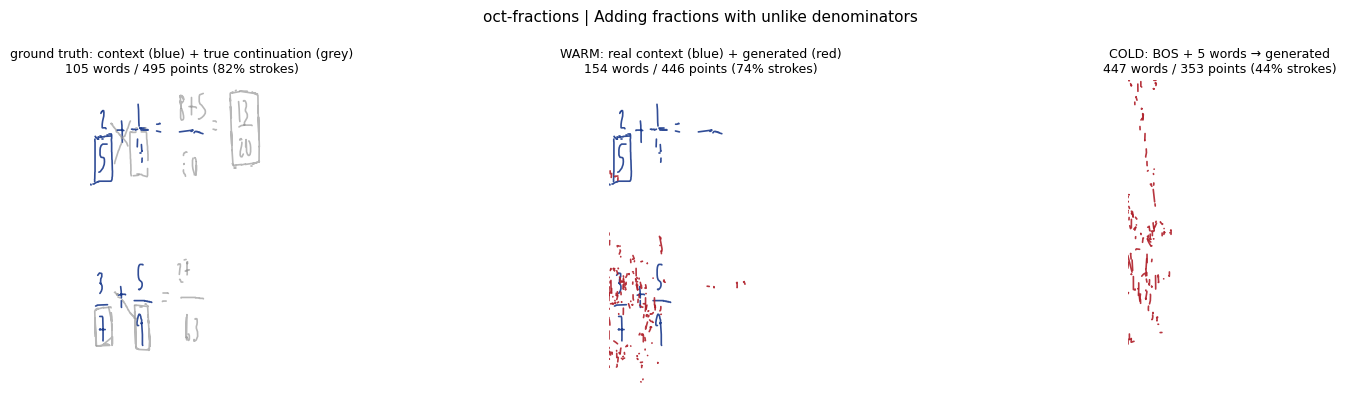
\includegraphics[width=\textwidth]{fig/gen_fractions.png}
    \caption{\emph{Adding fractions with unlike denominators.} Left: the real lecture --- context in blue, what actually came next in grey (two fraction problems with boxed answers). Middle: the same real context, then 600 tokens generated by the model in red. The scatter sits where the second problem really goes, but nothing in it is a digit. Right: generating from just the first five words.}
    \label{fig:gen1}
\end{figure}

\begin{figure}[ht!]
    \centering
    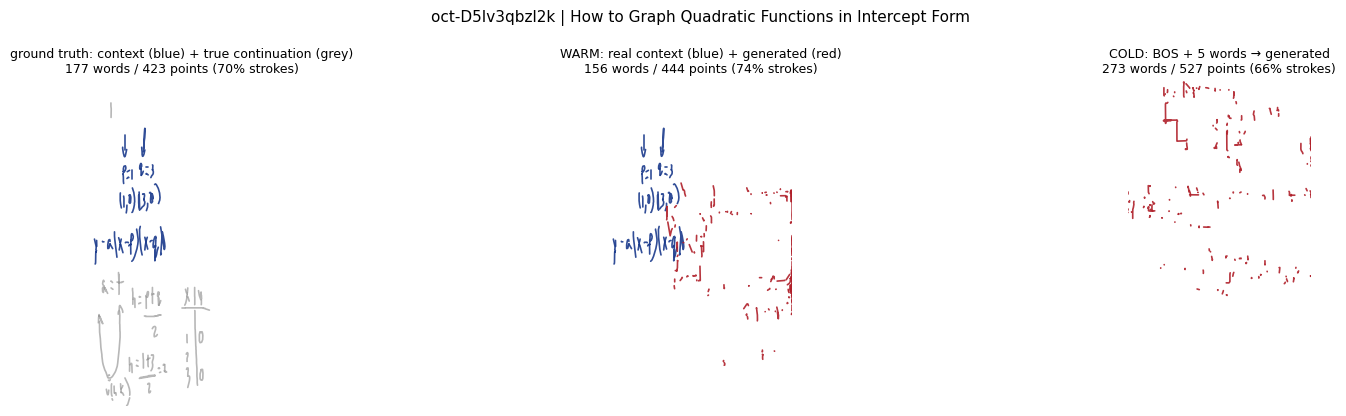
\includegraphics[width=\textwidth]{fig/gen_quadratic.png}
    \caption{\emph{Graphing quadratic functions in intercept form.} Same layout. The real page has an equation, a vertex formula and a table of $x$/$y$ values; the generated page has neither a curve nor a character.}
    \label{fig:gen2}
\end{figure}

Part of this is the usual gap between predicting one step with the true history and generating hundreds of steps from your own output: small errors feed back and compound~\citep{bengio2015scheduled,ranzato2016sequence}. But the bigger reason is what the data does not contain. It is not that the data is too small: pen loss was still falling at the last epoch in all 21 runs, and the corpus is larger than what the classic handwriting models were trained on. What the data lacks is a label saying \emph{which symbol is being drawn}. Graves' model produced readable cursive because it was told the character string and attended to it while writing~\citep{graves2013generating}; the systems that separate content from style make the same point from the other side~\citep{aksan2018deepwriting}. Here the only clue to the content is the speech, and finding~3 says the speech is not a usable clue at this size. The model learned how a pen moves, not what it is writing.

\section{Limitations}
\label{sec:limits}

\begin{enumerate}[leftmargin=*,itemsep=2pt]
\item \textbf{Small model.} 4.6M parameters. A larger model could learn to ignore the pen tokens, shrinking cost~2 until benefit~1 wins --- Chameleon reports that early fusion works at 7B and above~\citep{chameleon2024}. All results are ``at this scale''.
\item \textbf{One rung of the stroke ladder is not perfectly clean.} The \cond{<silent>} token stays visible in \cond{mask\_words} and \cond{noword\_hidden} but is removed in \cond{drop\_words}, so the last row of Table~\ref{tab:deltas} includes the value of that marker, not just spacing.
\item \textbf{Seed spread.} The three seeds agree on sign and their intervals do not overlap zero, but the magnitudes vary 2--3$\times$. The ranges are more honest than the means.
\item \textbf{Alignment noise.} Attaching strokes to words by time overlap is approximate. Some pairs are wrong, which would make finding~1 look smaller and finding~3 look closer to zero than they really are.
\item \textbf{No board clears.} Every video is treated as one page, so ``where things are on the board'' is only meaningful locally.
\end{enumerate}

\section{Next: an agent that plans what to say and what to draw}

The experiment says two things about how to build the real system. The information linking speech and drawing is real (finding~1), and the data is missing the one thing a drawing model needs most --- an explicit statement of \emph{what} to draw (finding~3 and the generation failure). A flat stroke model tries to discover that from correlation and cannot. So the next design supplies it directly.

The plan is a \textbf{language-model agent that writes the lecture as a script}: for each step, what to say, and what to put on the board --- a shape, an equation, a diagram, a label --- with where to put it. Something like:

\begin{center}
\small
\begin{tabular}{@{}l l@{}}
\toprule
say & draw \\
\midrule
``Let's add two fifths and one fourth.'' & \texttt{fraction 2/5 at (0.15, 0.20)}; \texttt{symbol + at (0.27, 0.22)}; \texttt{fraction 1/4 at (0.32, 0.20)} \\
``The denominators are different, so we need a common one.'' & \texttt{underline denominators}; \texttt{text ``LCD = 20'' at (0.15, 0.40)} \\
``Five times four is twenty.'' & \texttt{arrow from (0.17, 0.26) to (0.20, 0.38)} \\
\bottomrule
\end{tabular}
\end{center}

The agent decides the content and the layout; a renderer turns the drawing commands into strokes on a canvas. This is the pattern that has worked for diagrams~\citep{zala2024diagrammergpt}, page layouts~\citep{feng2023layoutgpt} and scientific figures~\citep{belouadi2024automatikz}, and SketchAgent showed that a frontier model can place strokes on a coordinate grid competently when the coordinates are given as a small vocabulary rather than raw numbers~\citep{vinker2024sketchagent}. Running it as a loop --- plan a step, render it, look at the board, plan the next~\citep{yao2023react} --- gives the agent the visual memory of the board that the flat model never had. It also separates the two jobs the flat model was forced to do at once, which is exactly what finding~2 says to do: keep the language reasoning in a stream that is all language, and give the drawing side an explicit instruction instead of asking it to guess from the words --- the Flamingo-style division of labour~\citep{alayrac2022flamingo} rather than the Chameleon-style one.

What the dataset from Section~\ref{sec:data} contributes to this: the aligned transcripts are the examples of \emph{how} this teacher structures an explanation --- what he says first, when he pauses to write, how much he draws per sentence --- and the extracted strokes are the reference for the layout conventions (where problems start, how far apart lines go) and, later, for rendering the primitives in his handwriting rather than a font, where the current text-to-ink models~\citep{pan2026diffink} are the natural tool. The evaluation would ask two things the current model could not be asked: does the drawing match what is being said, and does the layout stay readable as the lecture goes on.

\vspace{1em}
\noindent{\small\color{muted} Experiment numbers from \texttt{ctx\_ablation\_v2/} (7 conditions $\times$ 3 seeds, 363 held-out windows, 3,000 bootstrap resamples). The full design, the first run, and every bug found along the way are documented in \texttt{METHOD1\_CONTEXT\_EXPERIMENT.md}.}

\bibliographystyle{unsrtnat}
\bibliography{references}

\end{document}
